% \documentclass[]{ijsra}
% \newfontfamily\tamilfont[Ligatures=TeX]{NotoSerifTamil-Regular}

\def\IJSRAidentifier{\currfilebase} %<---- don’t change this!
\def\submission{}%YYYY-MM-DD
\def\acceptance{}%YYYY-MM-DD
%-------Title | Email | Keywords | Abstract-------------
\def\shorttitle{Indo-Roman Trade at Arikamedu}
\def\maintitle{Indo-Roman Trade at Arikamedu: \\
	A contextual analysis of finds from the UCL Institute of Archaeology Collection}
\def\cmail{ashwini.narayan94@gmail.com}
\def\keywords{Roman Trade, Southern India, Beadmaking, Trading networks, Indian Ocean}
%\def\keywordname{}%<--- redefine the name “Keywords“ in needed language
\def\abstract{Excavations conducted at Arikamedu by Sir Mortimer Wheeler revealed amphorae of Mediterranean origin as well as both imported and locally produced ceramics with Mediterranean-inspired \enquote{rouletted} decorations. It was concluded that Arikamedu was a trading post during the reign of Augustus.

The Periplus of the Erythraean Sea shows that the kingdoms of the Indian Ocean region were increasingly growing in wealth and importance due to the significant development of trading networks during Roman times. Nonetheless, in the case of Arikamedu, I argue that Mediterranean trade had long existed prior to Augustus' reign. This essay focuses on the ceramic evidence, together with other imported material, in order to study the nature and continuity of trade between Arikamedu and the Roman world and assess its socio-economic implications.}
%--------Author’s names------------
\def\authorone{Ashwini Lakshminarayanan}
%-------Biographical information-------------
\def\bioone{Ashwini Lakshminarayanan attends the International Hellenic University in Thessaloniki, Greece. She has completed a Master’s degree in Classical Archaeology and Ancient History of Macedonia. This article is a product of a Bachelor’s degree archaeological project on finds analysis from Arikamedu submitted at the University of Kent and supervised by Dr.~Ada Nifosi. Ashwini’s interests include Indo-Greek and Indo-Roman relations as well as female figures in South Asian art.}
%------University/Institution--------------
\def\affilone{International Hellenic University}

\begin{filecontents}{\IJSRAidentifier.bib}

@article{ardika1991,
	author = {Ardika, I. W. and Bellwood, P.},
	journal = {Antiquity},
	pages = {221-232},
	title = {Sembiran: the beginnings of Indian contact with Bali},
	volume = {247},
	year = {1991},
}
@incollection{bagnall2000,
	address = {Bruxelles},
	author = {Bagnall, R.S.},
	title = {Introduction},
	booktitle = {Documents from Berenice Volume I},
	editor = {Bagnall, R.S. and Helms, C., And Verhoogt, A.M.F.W.},
	publisher = {Fondation égyptologique Reine Élisabeth},
	year = {2000},
	page = {1-8},
}
@article{begley1983,
	author = {Begley, V.},
	journal = {American Journal of Archaeology},
	pages = {461-81},
	title = {Arikamedu Reconsidered},
	volume = {87},
	year = {1983},
}
@book{begley1986,
	author = {Begley, V.},
	publisher = {Expedition Magazine},
	title = {Rouletting and Chattering},
	year = {1986},
}

@article{begley1988,
	author = {Begley, V.},
	journal = {American Journal of Archaeology},
	pages = {427-440},
	title = {Rouletted Ware at Arikamedu: A New Approach},
	volume = {92},
	number = {3},
	year = {1988},
}

@techreport{begley1996,
	author = {Begley, V. and others},
	institution = {Centre d'histoire et d'archéologie, École française d'Extrême-Orient, Paris},
	title = {The Ancient port of Arikamedu: new excavations and researches 1989-1992, Part 1},
	year = {1996},
}

@incollection{begley2004,
	address = {Pondichéry},
	author = {Begley, V.},
	booktitle = {Ancient port of Arikamedu new excavations and researches, 1989-1992, Volume 1},
	publisher = {Centre d'histoire et d'archéologie, École française d'Extrême-Orient},
	year = {2004},
	page = {1-8},
}

@book{bushnell1998,
	author = {Bushnell, T.},
	publisher = {The Internet Classics Archives},
	title = {Res Gestae Divi Augusti},
	year = {1998},
}
@book{casson1989,
	address = {New York},
	author = {Casson, L.},
	publisher = {Princeton University Press},
	title = {The Periplus Maris Erythraei: Text with Introduction, Translation and Commentary},
	year = {1989},
}
@article{chami2001,
	author = {Chami, F. A.},
	journal = {Man and Environment},
	number = {1},
	pages = {33-44},
	title = {People and contacts in the ancient western Indian Ocean seaboard or Azania},
	volume = {27},
	year = {2001},
}
@book{champakalakshmi1996,
	address = {New Delhi},
	author = {Champakalakshmi, R.},
	publisher = {Oxford University Press},
	title = {Trade, Ideology and Urbanisation: South India, 330 BC to AD 1300},
	year = {1996},
}
@book{chandra1977,
	address = {New Delhi},
	author = {Chandra, M.},
	publisher = {Abhinav Publications},
	title = {Trade and Trade Routes in Ancient India},
	year = {1977},
}
@book{correspondent2007,
	author = {Correspondent, S.},
	publisher = {The Hindu. [Online]},
	year = {2007},
}
@article{charlesworth1928,
	author = {Charlesworth, M.P.},
	year = {1928},
	title = {Some Notes On the Periplus Maris Erythraei},
	journal = {Classical Quarterly},
	volume = {22},
	number = {2},
	pages = {92-100},
}
@book{craik2015,
	address = {London},
	author = {Craik, E.},
	publisher = {Routledge Revivals},
	title = {The Dorian Aegean},
	year = {2015},
}
@book{dihle1965,
	author = {Dihle, A.},
	year = {1965},
	title = {Umstrittene Daten Untersuchungen zum Auftreten der Griechen am Roten Meer: Das Datum des Periplus des Roten Meeres},
	address = {Koln},
	editor = {Dihle, A.},
}
@book{dressel1899,
	address = {Berlin},
	author = {Dressel, H.},
	title = {Corpus Inscriptionum Latinarum, band XV},
	year = {1899},
}
@article{empereur1989,
	author = {Empereur, J. Y. and M. Picon.},
	journal = {ARHE},
	pages = {223-248},
	title = {Les régions de production d'amphores impériales en Méditerranée orientale},
	year = {1989},
}
@book{frakes2009,
	address = {Vienna},
	author = {Frakes, J. F.},
	publisher = {Phoibos},
	title = {Framing Public Life: The Portico in Roman Gaul},
	year = {2009},
}

@article{francis1986,
	author = {Francis Jr, P.},
	journal = {Bulletin of the Deccan College Post-Graduate \& Research Institute},
	pages = {117-121},
	title = {Collar beads: a new typology and a new perspective on ancient Indian beadmaking},
	volume = {45},
	year = {1990},
}

@article{francis1990,
	author = {Francis Jr, P.},
	journal = {Asian Perspectives},
	number = {1},
	pages = {1-23},
	title = {Glass Beads in Asia, Part 2: Indo-Pacific Beads},
	volume = {XXIX},
	year = {1990},
}
@incollection{francis2000,
	address = {Leiden},
	author = {Francis Jr, P},
	booktitle = {Report of the 1998 excavations at Berenike and the survey of the eastern desert including excavations at the Wadi Kalat.},
	editor = {Sidebotham, S. E. and Wendrich, W. Z},
	publisher = {CNWS},
	title = {Human Ornaments},
	year = {2000},
}
@book{francis2002,
	address = {Honolulu},
	author = {Francis Jr, P.},
	publisher = {University of Hawaii Press},
	title = {Francis: Asia's Maritime Bead Trade},
	year = {2002},
}
@incollection{francis2007,
	address = {Los Angeles},
	author = {Francis Jr, P.},
	booktitle = {Berenike 1999/2000: Report on the excavations at Berenike including Wadi Kalat and Siket and the survey of the Mons Smaragdus Region},
	editor = {Sidebotham, S. E and Wendrich, W. Z},
	publisher = {University of California},
	title = {Personal adornments},
	year = {2007},
}
@article{gwinett1988,
	author = {Gwinett, A. and Gorelick, L.},
	journal = {Archaeomaterials},
	number = {2},
	pages = {183-93},
	title = {A possible lapidary training piece from Arikamedu, India},
	volume = {2},
	year = {1988},
}
@article{haerinck1998,
	author = {Haerinck, E.},
	journal = {Akkadica},
	pages = {22-40},
	title = {The shifting pattern of overland and seaborne trade in SE-Arabia: foreign pre-Islamic coins from Mleiha},
	year = {1998},
}
@article{harrauer1985,
	author = {Harrauer, H. and Sipjesteijen, P.},
	journal = {Anzeiger der Österreichischen Akademie der Wissenschaften, Phil.-Hist. Klasse},
	pages = {124-155},
	title = {Ein neues Dokument zu Roms Indienhandel, P. Vindob. G 40822},
	volume = {122},
	year = {1985},
}
@incollection{harrell1996,
	address = {Leiden},
	author = {Harrell, J. A.},
	booktitle = {Berenike 1995: Preliminary Report on the 1995 Excavations at Berenike (Egyptian Red Sea Coast) and the Survey of the Eastern Desert},
	editor = {Sidebotham, S. E. and W. Z. Wendrich},
	pages = {99-126},
	publisher = {Centre for Non-Western Studies, Leiden University},
	title = {Geology},
	year = {1996},
}
@book{howard2012,
	address = {Jefferson},
	author = {Howard, M. C.},
	publisher = {McFarland},
	title = {Transnationalism in Ancient and Medieval Societies: The Role of Cross-Border Trade and Travel},
	year = {2012},
}
@book{jones1917,
	address = {London},
	author = {Jones, H.},
	publisher = {Loeb Classical Library},
	title = {Strabo's Geography},
	year = {1917},
}
@book{kamalakar2000,
	address = {New Delhi},
	author = {Kamalakar, G.},
	publisher = {Bharatiya Kala Prakashan},
	title = {South Indian Archaeology},
	year = {2000},
}
@incollection{kasinathan1994,
	address = {Madras},
	author = {Kasinathan, N.},
	booktitle = {Collected Papers (Studies in Tamil Culture)},
	editor = {Kacinatan, N.},
	pages = {31-34},
	publisher = {State Department of Archaeology},
	title = {Two Roman Coins from Alagankulam Excavation},
	year = {1994},
}

@incollection{kasinathan1996,
	address = {New Delhi},
	author = {Kasinathan, N.},
	booktitle = {Gauravam. Recent Researches in Indology},
	editor = {Kasinathan, N.},
	pages = {86-92},
	publisher = {Herman Publishing House},
	title = {A Preliminary Report on the Excavations at Alagankulam, Tamilnadu},
	year = {1996},
}

@book{lannoye2015,
	address = {North Charleston},
	author = {Lannoye, V.},
	publisher = {CreateSpace Independent Publishing Platform},
	title = {The History of Money for Understanding Economics},
	year = {2015},
}
@book{laubenheimer1990,
	address = {Paris},
	author = {Laubenheimer, F.},
	publisher = {Errance},
	title = {Le temps des amphores en Gaule: vins, huiles et sauces},
	year = {1990},
}
@book{mairs2016,
	address = {Berkeley},
	author = {Mairs, R.},
	publisher = {University of California Press},
	title = {The Hellenistic Far East: Archaeology, Language, and Identity in Greek Central Asia},
	year = {2016},
}
@incollection{mahadevan1995,
	address = {Leiden},
	author = {Mahadevan, L.},
	booktitle = {Preliminary Reports of the 1995 Excavation at Bernike},
	pages = {731-45},
	publisher = {CNWS},
	title = {Tamil Brahmi Graffito},
	year = {1995},
}
@article{newbold1844,
	author = {Newbold,C.},
	journal = {Journal of the Asiatic Society},
	pages = {20-37},
	title = {Summary of the geology of Southern India},
	volume = {IX},
	year = {1844},
}
@incollection{nagappan1974,
	author = {Nagappan Nayar, K. and Mahadevan, S.},
	booktitle = {The Commercial Mollusks of India},
	pages = {122-140},
	publisher = {Central Marine Fisheries Research Institute Cochin Bulletin, Volume 25},
	title = {Chank Fisheries and the Industrial use of Chank},
	year = {1974},
}
@incollection{rajan1998,
	address = {New Delhi},
	author = {Rajan, K.},
	booktitle = {Tradition and Archaeology. Early Maritime contacts in the Indian Ocean. Proceedings of the International Seminar Techno-Archaeological Perspectives of Seafaring in the Indian Ocean 4th cent. B.C. - 15th cent. A.D.},
	editor = {Himanshu Prabha Ray and Jean-François Salles},
	publisher = {Manohar Publishers and Distributors},
	title = {Early maritime activities of the Tamils},
	year = {1998},
}
@book{ramachandran1980,
	address = {Delhi},
	author = {Ramachandran, K. S.},
	publisher = {Sandeep Prakashan},
	title = {Archaeology of South India: Tamil Nadu},
	year = {1980},
}
@article{redfern2016,
	author = {Redfern, R. and others},
	journal = {Journal of Archaeological Science},
	pages = {11-22},
	title = {Going south of the river: A multidisciplinary analysis of ancestry, mobility and diet in a population from Roman Southwark, London},
	volume = {74},
	year = {2016},
}

@book{sherwin-white1978,
	address = {Virginia},
	author = {Sherwin-White, S.},
	publisher = {Vandenhoeck \& Ruprecht GmbH KG},
	title = {Ancient Cos},
	year = {1978},
}

@book{sidebotham2008,
	address = {Cairo},
	author = {Sidebotham, S. and M. Hense and H. Nouwens},
	publisher = {American University in Cairo Press},
	title = {The Red Land: The Illustrated Archaeology of Egypt's Eastern Desert},
	year = {2008},
}
@book{sinkankas1996,
	address = {New Delhi},
	author = {Sinkankas,J.},
	publisher = {Affiliated East-West Press},
	title = {Mineralogy: A First Course},
	year = {1996},
}
@book{sharma2002,
	address = {New Delhi},
	author = {Sharma, P. and Yelne, M. and Dennis, J.},
	publisher = {Central Council for Research in Ayurveda and Siddha},
	title = {Database on Medicinal Plants Used in Ayurveda 5},
	year = {2002},
}
@article{smith2002,
	author = {Smith, M.},
	journal = {Man and Environment},
	number = {1},
	pages = {139-51},
	title = {The Role of Local Trade Networks in the Indian Subcontinent in the Early Historic Period},
	volume = {XXVII},
	year = {2002},
}
@article{suresh2010,
	author = {Suresh, S.},
	journal = {Minerva},
	number = {5},
	pages = {28-31},
	title = {Rome's sea Route to India},
	volume = {21},
	year = {2010},
}
@book{tchernia2016,
	address = {Oxford},
	author = {Tchernia, A.},
	publisher = {Oxford University Press},
	title = {The Romans and Trade},
	year = {2016},
}
@article{tomber2012,
	author = {Tomber, R.},
	journal = {British Museum Studies in Ancient Egypt and Sudan},
	pages = {201-215},
	title = {From the Roman Red Sea to beyond the Empire: Egyptian ports and their trading partners},
	volume = {18},
	year = {2012},
}
@book{turner1989,
	address = {London},
	author = {Turner, P.},
	publisher = {Institute of Archaeology Occasional Publication 12},
	title = {Roman Coins from India},
	year = {1989},
}

@book{turner2016,
	address = {London},
	author = {Turner, P.},
	title = {Roman Coins from India},
	year = {2016},
}

@book{thapar2002,
	address = {London},
	author = {Thapar, R.},
	publisher = {Penguin Books},
	title = {Early India from the Origins to AD 1300},
	year = {2002},
}
@incollection{vanderveen,
	address = {Southampton},
	author = {Van der Veen, M.},
	booktitle = {Myos Hormos and Queseir Al Qadim: A Roman and Islamic Port on the Red Sea coast of Egypt: Interim Report 2001},
	editor = {Peacock, D., Blue and L., Moser},
	publisher = {University of Southampton},
	title = {The plant remains: diet and fuel in Roman Myos Hormos},
	year = {2001},
}%source not used
@book{virgil,
	author = {Virgil},
	editor = {Dryden, J.},
	publisher = {The Internet Classics Archives},
	title = {The Aneneid},
	year = {n.d.},
}
@article{wheeler1946,
	author = {Wheeler, M. and others},
	journal = {Ancient India},
	pages = {17-25},
	title = {Arikamedu, an Indo-Roman Trading Station on the East Coast of India},
	volume = {2},
	year = {1946},
}
@book{wheeler1954,
	address = {New York},
	author = {Wheeler, M.},
	title = {Rome beyond the Imperial Frontiers},
	year = {1954},
}
@book{wheeler1955,
	address = {London},
	author = {Wheeler, M.},
	publisher = {Bell},
	title = {Rome beyond the Imperial Frontiers},
	year = {1955},
}
@article{whitcomb1996,
	author = {Whitcomb, D.},
	journal = {Topoi},
	pages = {747-72},
	title = {Quesar Al Qadim and the Location of Myos Hormos},
	volume = {6},
	year = {1996},
}
@book{whitcomb1982,
	address = {Cairo},
	author = {Whitcomb, D. and Johnson, J. H.},
	publisher = {Undena Publications},
	series = {American Research Center in Egypt Reports 7},
	title = {Quesar Al Qadim 1980 Report},
	year = {1982},
}

@book{whittaker1994,
	address = {Baltimore},
	author = {Whittaker, C.},
	publisher = {Johns Hopkins University Press},
	title = {Frontiers of the Roman Empire: A Social and Economic study},
	year = {1994},
}
@incollection{will1992a,
	address = {Boulder},
	author = {Will, E.},
	booktitle = {Ceramic Production and Distribution: An intergrated approach},
	editor = {Beyll, G.J. and Pool, C.},
	publisher = {Westview},
	title = {Production, Distribution, and Disposal of Roman Amphorae},
	year = {1992a},
}
@book{will1992b,
	address = {Paris},
	author = {Will, E.},
	publisher = {Collins},
	title = {Les Palmyreniens: Venice des sables},
	year = {1992b},
}
@article{will2001,
	author = {Will, E.},
	journal = {American Journal of Archaeology},
	number = {2},
	pages = {263},
	title = {Truth in Roman Labeling?},
	volume = {105},
	year = {2001},
}
@article{zlateva2015,
	author = {Zlateva, B. and Rangelov, M.},
	journal = {Journal of Applied Spectroscopy},
	number = {2},
	pages = {221-227},
	title = {Chemical Analysis of Organic Residues Found in Hellenistic Time Amphorae from South East Bulgaria},
	volume = {82},
	year = {2015},
}

\end{filecontents}
\IJSRAopening%<---- don’t change this!
%-------
\IJSRAsection{Introduction}

\lettrine{T}{he} port city of Arikamedu is located on the Ariyankuppam lagoon, in the Southeastern coast of India. The Gingee river connects it to the Bay of Bengal, which provide access to the Indian Ocean (\cref{fig:Lakshminarayanan_Figure_01}). The area surrounding Arikamedu has several sea inlets and backwaters, thus making it a suitable location for harbouring ships safely. Arikamedu is often identified as the “Poduke Emporium” in the \emph{Periplus}. In this paper, I discuss the proactive role of this trading port in Indo-Roman trading networks.

%FIGURE 01: Map
\begin{figure}[!htb]
	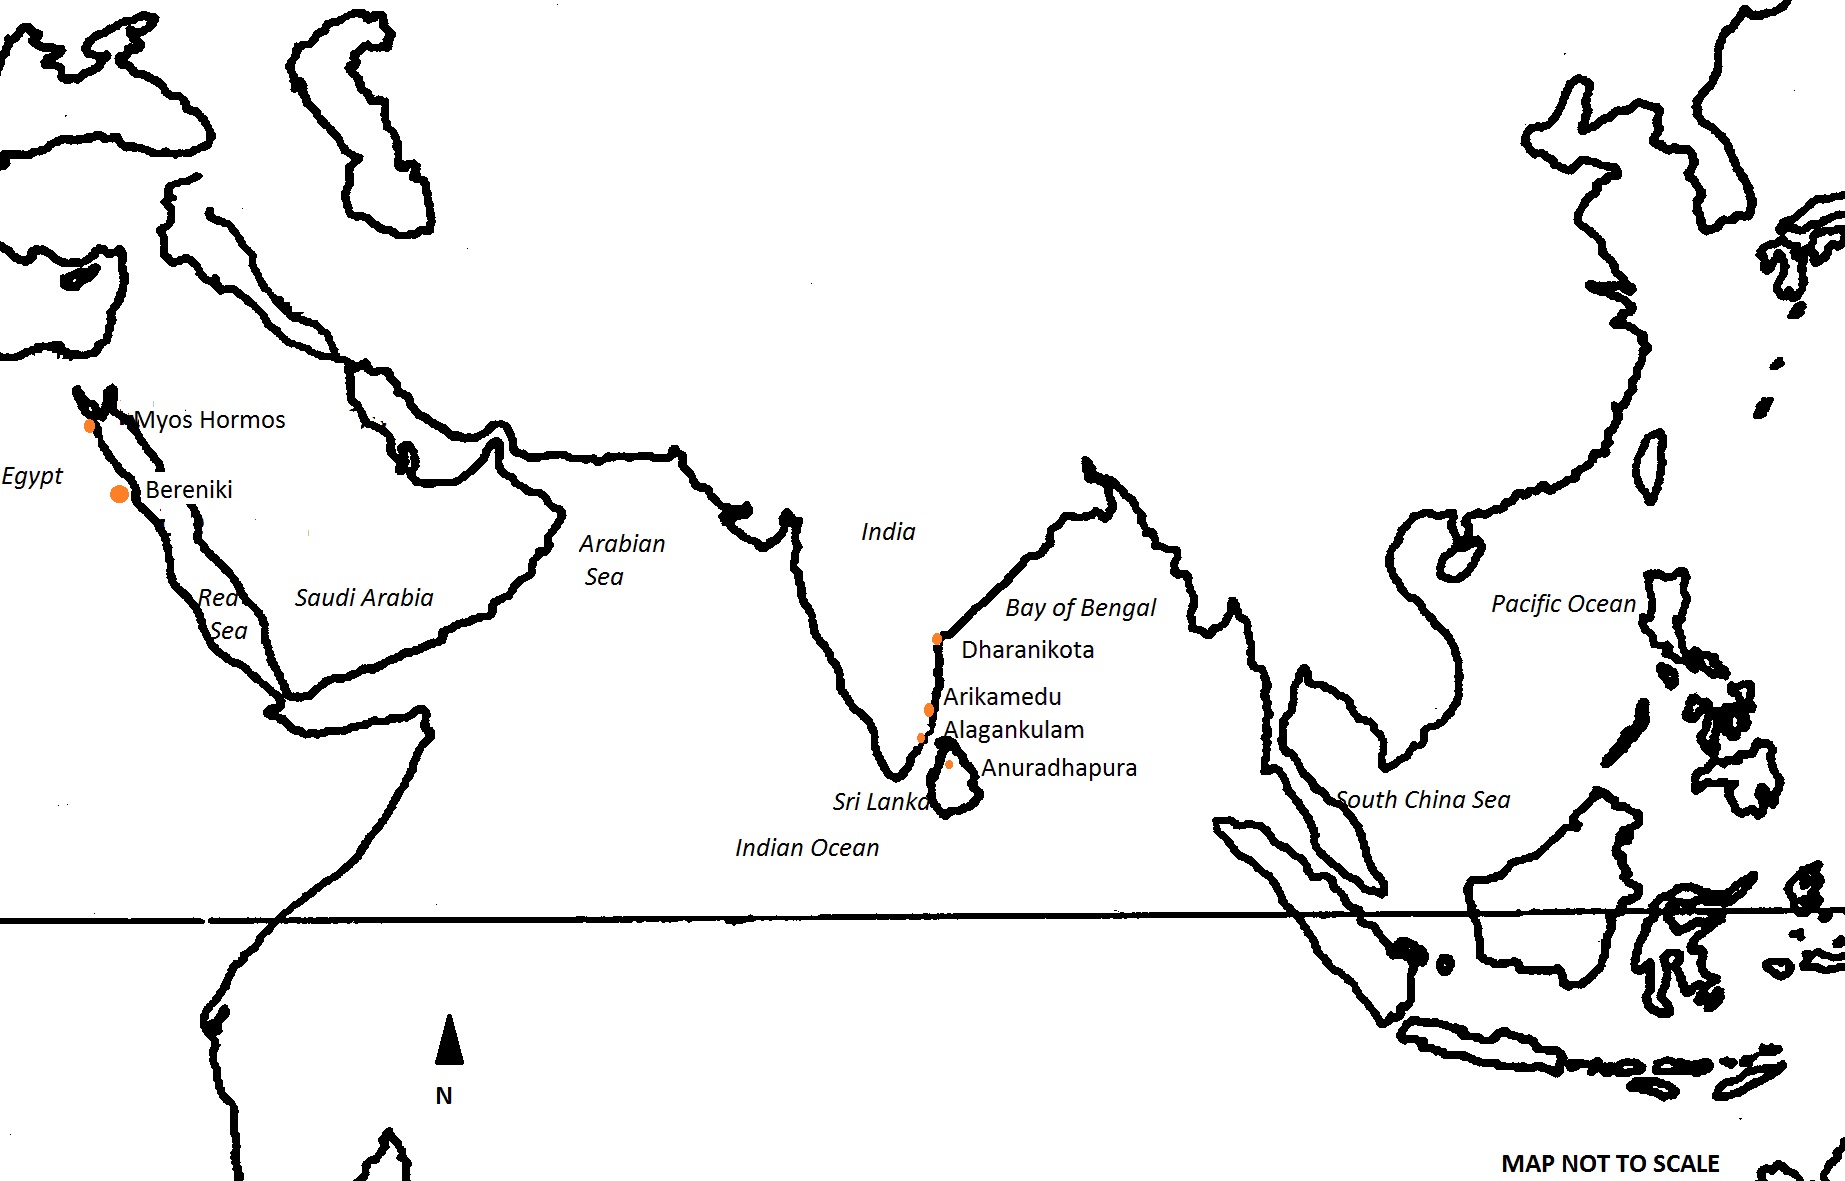
\includegraphics[width=\linewidth]{Lakshminarayanan_Figure_01}
	\caption{Map of the Indian Ocean with the sites mentioned in this paper\\
		{\normalfont\scriptsize\copyright\
			\shortauthor, illustration
	}}
	\label{fig:Lakshminarayanan_Figure_01}
\end{figure}

The medieval \emph{mappamundi}, the map of the world, was commissioned by Emperor Augustus to survey the world. The map encapsulates the political visions of the imperial power. Augustus’ empire was indeed considered “\emph{imperium sine fine}” (Virgil, Aeneid.279) mainly because of its prosperity, which were partly due to booming trade relationships. The Roman conquest of Egypt improved access to the Indian Ocean world, and a more efficient sea route was established between Rome and India via Egypt. Strabo recounts that by this time (year 26), a hundred and fifty ships sailed to India each year via southern Egypt (Strabo, \emph{Geography}, 2.5:12). In this respect, the port of Arikamedu is particularly important for understanding the trade between Rome and India via Egypt.

India was seen as an ‘imperial province’ and Tamil kings were amongst the ambassadors who visited Augustus (Pandion King, Strabo, \emph{Geography}, 15.1:4). Ambassadors from Indian kingdoms frequenting Augustus’ court was a “thing never seen before” (Aug. \emph{Res Gestae}: 31). Although Rome had no political power in India, the Romans believed that their sovereignty extended to these countries and that Rome had the right to intervene and expect obedience from them \parencite[][34-37]{whittaker1994}.

Augustus’ knowledge of India can only be derived from literary sources that are available to us, such as Ovid (Ov. Medic. 10), Horace (Odes 1.12.3-57, 1.31.6), Virgil (Geo. 157), and prose writers such as Diodorus (2.35.41). Strabo accounted that the trade between Rome and India began after the annexation of Egypt. The stories were rather fantastic, with only a few literary sources containing indubitable information pertaining to mercantile trade. Such an account is the \emph{Periplus of the Erythraen Sea}. This work contains valuable information about navigational routes and trading ports, and is crucial for developing an inventory of items that were traded across the Indian Ocean. The text has not been dated accurately but many scholars believe that it was written the middle of the 1st century\AD \parencite[][98]{charlesworth1928}.%missing reference!
A reference in the text to a Nabataean King named Malichus has been identified as referring to Malichus II, who reigned around 40-70\AD and this identification puts the text around the same period (\emph{PME} 19, \cite[][9-35]{dihle1965}.%missing reference!

According to the \emph{Periplus}, ships from the Roman Empire set out in two different routes, one to Africa and the other to India. The ships would leave the Red Sea in July in order to catch the monsoonal currents, easing the long and dangerous voyage to India (\emph{PME} 14). These ships, after procuring the goods, left the ports of India between December and January. The materials sold to Indian traders include wine, glass, metal, coral, textiles, Roman money, and frankincense. The Romans, in return, purchased bdellium, nard, precious stones, ivory, cotton, cloth and silk. The main exports were pepper, Malabathron, Chinese silk, and gemstones. The \emph{Periplus} mentions that large amounts of Roman money were spent in India to procure these luxurious goods, and many Roman coins have indeed been found in India (170 finds from 130 different sites), dating from the Augustan to Tiberian periods \parencite[][]{turner1989}. It should be noted that the number of Roman coins found in both the Krishna Valley (Andhra Pradesh) and the Coimbatore area of Tamil Nadu is significantly higher than those found elsewhere in the sub-continent (\cref{fig:Lakshminarayanan_Figure_18}).

In early Tamil society, poems and anthologies based on popular social themes were compiled into the Sangam corpus. The Sangam literary corpus refers to foreign ships sailing to the coast of Tamil Nadu, and the consumption of Italian wine. The foreigners were termed \emph{Yavanah} in contemporary literary works. This term may refer to people from the Mediterranean, African and Arabian regions, thus indicating a strong network of merchant traders arriving at the ports of South India. Indigenous Tamil works give detailed accounts of the importance of imported goods and their places of origin. The \emph{Akananooru}, a tamil poetic work on love and separation, speaks about the \emph{Yavanah} wine that was exchanged for rare products of the sea. It also states that when the \emph{Yavanah} ships come, they leave full of black pepper. The \emph{Pattupattu}, written between 200 \BC to\AD 300 \parencite[][231]{thapar2002}, compares the noise made by the loading and unloading of cargo into large Roman ships with that of the noise made by weavers.

\begin{quote}
{\tamilfont
யவனர் தந்த வினை மாண் நன்கலம்\\
பொன்னொடு வந்து கறியொடு பெயரும்\\
வளங் கெழு முசிறி ஆர்ப்பெழ வளஇ}\\[.5em]
(Ettuthogai; {\tamilfont அகநானூறு} 149 lines  9-11)\\
Trans.: \emph{The Yavanas come in fine ships bearing gold and leave with black pepper into Muchiri town}
\end{quote}

Consumption of wine rather than the local toddy is also mentioned in Tamil literature.
\begin{quote}
{{\tamilfont மட்டு நீக்கி மது மகிழ்ந்தும்}}\\[.5em]
(Pattupattu, Pattinappalai: 108)\\
Trans.: \emph{Drink wine instead of palm toddy}
\end{quote}
Accurately dating these literary works is difficult, as they are part of a much older tradition passed down purely through oral traditions. It is, therefore, impossible to say with any certainty that these works can be dated to the first century\AD.

The artefacts analysed in this article are currently housed in the University College of London’s Institute of Archaeology. The type of artefacts considered here provides a better understanding of the range of products that were being traded. Analysing the typology of amphorae and table ware found at the site enables us to compare goods mentioned in literary sources to the archaeological material, while also facilitating the dating of the site. Correlating fragmentary literary and archaeological data is challenging, but it can provide a balanced narrative. Moreover, excavation reports and published literature based on the reports has also been used here as secondary sources. The aim of the study is to understand the scope and importance of Arikamedu in Roman trade based on the import and export of diverse goods. Recent research, including the preliminary analysis of bones from individuals of potential Chinese origin found in the Southwark area (London) suggests that these individuals likely lived between the 2\textsuperscript{nd} and 4\textsuperscript{th} century\AD \parencite{redfern2016} have highlighted Indo-Roman relationships. Improving our understanding of the socio-economic relationships between Asia and the Roman empire is thus paramount. I would argue that the traditional conceptualisation of the nature of these relationships as occasional or minor needs to be thoroughly reconsidered in order to allow for a better understanding of the interconnectivity between regions in the ancient world.

\IJSRAsection{Excavations}

Prior to Wheeler’s excavation, French and Indian archaeologists had already identified Italian red glazed Arrentine ware and amphorae from the Mediterranean. His excavation at Arikamedu in 1945 was significant for identifying a port named in the \emph{Periplus}, thus improving our understanding of Indo-Roman connections (\cref{fig:Lakshminarayanan_Figure_02} and \cref{fig:Lakshminarayanan_Figure_03}). Based on the available evidence, Mortimer Wheeler suggested that the trading post in Arikamedu was active during the first two centuries\AD.

Following the \emph{Archaeological Survey of India} and Wheeler’s systematic excavation, Jean-Marie Casal investigated the site in 1947-8. The finds from this excavation were published in the monograph \emph{Fouilles de Virampatnam-Arikamedu; rapport de l'Inde et de l'Occident aux environs de l'ère chrétienne}. The occupation near the north and south banks of the site shows that the area was primarily inhabited by fishing communities. The port received a wide variety of wines, cut gems, Roman lamps, glass, and other table wares. During the booming trade, the fishing village developed into a brick built town, spreading northwards. The site also shows a large brick structure, which was over \num{150} feet long, suggesting the existence of a warehouse (see \cref{fig:Lakshminarayanan_Figure_02}). In the south, excavations revealed a courtyard walled with timber and brick, wells and soak-pits, with superimposed terracotta rings. The industrial quarters were found further south, yielding several containers and piping system for the supply and drainage of effluents and dyes. Wheeler hypothesised that here the muslins were dyed, and beads and objects made of semi-precious stones were assembled and finished \parencite{wheeler1946}. However, the dyeing facilities could not be confirmed by later excavations \parencite[][109]{begley1996}.

%FIGURE 02: Site plan
\begin{figure}[!htb]
	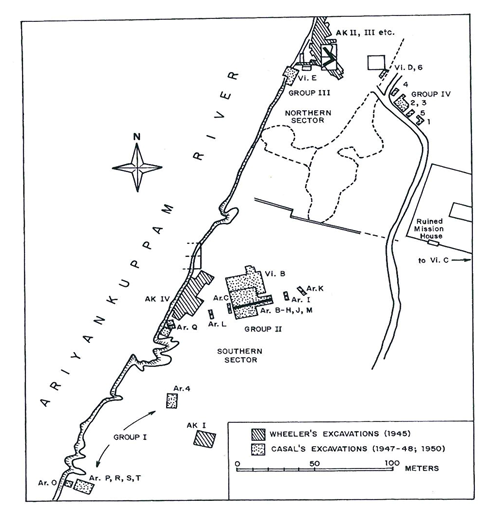
\includegraphics[width=\linewidth]{Lakshminarayanan_Figure_02}
	\caption{Site Plan of Arikamedu redrawn after J.-M. Casal (1956), from \textcite[][465]{begley1983}\\
		{\normalfont\scriptsize\copyright\ Reprinted with permission, courtesy of the Presses Universitaires de France.
	}}
	\label{fig:Lakshminarayanan_Figure_02}
\end{figure}

%FIGURE 03: Section plan
\begin{figure}[!htb]
	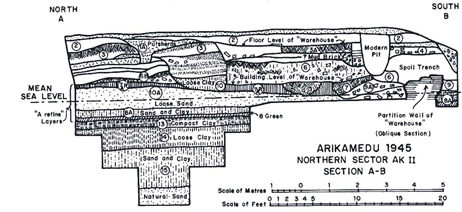
\includegraphics[width=\linewidth]{Lakshminarayanan_Figure_03}
	\caption{Section Plan of Arikamedu, after \textcite[][]{wheeler1946}\\
		{\normalfont\scriptsize\copyright\ Reprinted with permission, courtesy of Ancient India and Archaeological Survey of India \parencite[][468]{begley1983}.
	}}
	\label{fig:Lakshminarayanan_Figure_03}
\end{figure}

The subsequent layers after the expansion also yielded red pottery made in Arezzo. The layers also contained debris of ivory, iron, copper, and worked and unworked semi-precious stones.

All the strata in this excavation revealed amphorae sherds, together with at least fifty sherds of Arrentine ware, including fragments with pottery stamps (VIBIE, ITTA, CAMVRI, C. VIBI OF) \parencite[][177]{wheeler1955}. Other pieces of pottery were found near the “warehouse” where mercantile activities were likely conducted.

\IJSRAsection{Literary and Archaeological analysis of imports}

Literary evidence has shed much light upon the Roman presence in India. They suggest that the high point of trade between these two cultures was during the first century\AD. Relevant for archaeological research are the passing mention of goods in ancient literature that have been identified amongst the remains on the site. Works such as Pliny’s \emph{Natural History} or Strabo’s \emph{Geography} are significant because they narrate details on the area and sea routes to ports and cities mentioned in the \emph{Periplus}. The rich archaeological record of Arikamedu, evidencing intense trading activities, has been associated with Poduke. Poduke is named in the \emph{Periplus} (\emph{PME} 60) and in Ptolemy’s \emph{Geography} where it is mentioned once. According to these literary sources, it acted as a local harbour that received goods from other areas in India in the context of international trade rather than a harbour for direct overseas trade.

The pottery found in the excavation can be classified into two different types: amphorae and \emph{terra sigillata} ware. \emph{Terra sigillata} is a red glazed or orange-red coloured pottery with decorative moulding. This ware is also known as Arrentine ware and has an important manufacturing centre in Arrentinium (modern Arezzo, Italy). It is also called stamped pottery due to the mould stamps. It was widely used in Roman trade and was found in Arikamedu. The 22 sherds identified in the stratified deposits are flat-base dishes and footed cups bearing potter stamps from Vibi, C. Amurius and P. Atticus \parencite[][21]{wheeler1946}. The import of wine amphorae began before the original manufacture of Arrentine ware, and continued much after the distribution of this ware ceased. This evidence suggests that Arikamedu was likely a trading port prior to the first century.

Amphorae are trading vessels used in antiquity to carry liquid products such as wine, vinegar, fish products, oil, and other items used in everyday life (\cref{fig:Lakshminarayanan_Figure_04} and \cref{fig:Lakshminarayanan_Figure_05}). Amphorae are transported for their contents and not for their purpose of utility. The amphorae itself is secondary, as value was only attached to the product it was carrying. The archaeological analysis of these vessels can provide insight into their content and area of manufacture. For example, scientific analysis of the residues absorbed by vessel as a consequence of prolonged storage can provide valuable information regarding its content.

%FIGURE 04: Ceramic
\begin{figure}[!htb]
	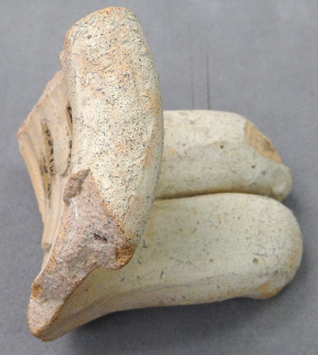
\includegraphics[width=\linewidth]{Lakshminarayanan_Figure_04}
	\caption{Ceramic Rim Fragment\\
		{\normalfont\scriptsize\copyright\ Courtesy of the UCL Institute of Archaeology Collections.
	}}
	\label{fig:Lakshminarayanan_Figure_04}
\end{figure}

%FIGURE 05: Amphora
\begin{figure}[!htb]
	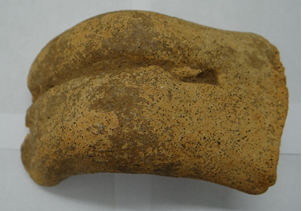
\includegraphics[width=\linewidth]{Lakshminarayanan_Figure_05}
	\caption{Amphora fragment\\
		{\normalfont\scriptsize\copyright\ Courtesy of the UCL Institute of Archaeology Collections.
	}}
	\label{fig:Lakshminarayanan_Figure_05}
\end{figure}

The composition of the clay and the type associated with it can provide information about the place of production. Moreover, some basic shapes of amphorae often relate to the product it contained. This pattern has assisted in the classification of amphorae types, such as the typology established by the Dressel table \parencite[][Pl III]{dressel1899}.

Nevertheless, the interpretation of amphorae from Arikamedu was not straightforward. This is due to the complicated nature of the trading networks, the presence of generic vessel types, together with minimal clay and residue analysis of sample types. Despite the problem regarding amphorae types, studies have revealed that some sherds show certain regional characteristic of Greek manufactures.

Several varieties of commercial amphorae found during the excavation suggest a Greco-Roman dimension. The clay analysis of the amphorae has revealed resin residue on the clay body which points towards the importation of Greek wine, because during the Hellenistic age, pine resin was deliberately added in the production of impermeable clays. It also aided in isolating moisture in the vessel (amphorae) that contained the wine, thus contributing to safeguarding the product in transoceanic trade \parencite[][222]{zlateva2015}.

One of the amphorae discovered in Arikamedu strongly resemble pottery from the Greek islands of Rhodes and Kos \parencite[][114]{begley2004}. This suggests that Koan wine was traded here as it was widely exported by Italian merchants to Asia and the Middle East in exchange for goods. The white Koan variety of wine tasted both sweet and salty, and this type was in demand in Rome and Eastern ports (Pliny. \emph{NH}. 14.78; \cite[][236-241]{sherwin-white1978}.%missing reference!
Athenaus and Pliny remark that Koan wine was mixed with sea water. Pliny and Virgil note that the wine was of superior quality (Strabo. 14. 2. 15; Pliny. \emph{NH} 14.10), although Athenaus considered Koan wine to have too much salt water in it (Ath. \emph{Deipnosophists}. 1). It is not possible to suggest whether Koan wine highly ranked in terms of quality, despite being widely circulated \parencite[][16]{craik2015}.

The Koan type (or Dressel 4) had thinner walls, small rim and a short neck. The Dressel 4 (Koan) type was efficient in maintaining the structure as well as having a better weight to capacity ratio compared to its counterparts \parencites[][229]{empereur1989}[][117]{laubenheimer1990}. Imitation Koan wine jars originating in Pompeii were shipped to India occasionally bearing the words COVM VET \parencite[][263]{will2001}. The place of production of this type can be identified in Kos, Knidos, Rhodes, Turkey, Italy, Spain, North Africa, and Nile Valley and a few organic storage jars from Hadramawt.

The spatial and density distribution patterns of amphorae found at Arikamedu suggests that significant amounts of wine were imported to the site. Although a majority of these amphorae jars found at Arikamedu contained wine, clay analysis suggests that some also carried olive oil or \emph{garum}, a type of fish sauce \parencite[][150]{will1992a}. Wares found in the region also resemble common Mediterranean tablewares (\cref{fig:Lakshminarayanan_Figure_06} and \cref{fig:Lakshminarayanan_Figure_07}) that are similar to those found in Gaul \parencite[][69]{frakes2009}. The assemblage has been dated between the second century \BC to the late first century\AD, so potentially starting before the Augustean period.

%FIGURE 06: Bowl
\begin{figure}[!htb]
	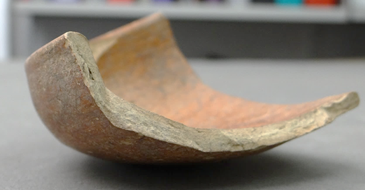
\includegraphics[width=\linewidth]{Lakshminarayanan_Figure_06}
	\caption{Fragment of a shallow bowl\\
		{\normalfont\scriptsize\copyright\ Courtesy of the UCL Institute of Archaeology Collections.
	}}
	\label{fig:Lakshminarayanan_Figure_06}
\end{figure}

%FIGURE 07: Ceramic 2
\begin{figure}[!htb]
	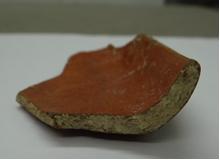
\includegraphics[width=\linewidth]{Lakshminarayanan_Figure_07}
	\caption{Ceramic fragment\\
		{\normalfont\scriptsize\copyright\ Courtesy of the UCL Institute of Archaeology Collections.
	}}
	\label{fig:Lakshminarayanan_Figure_07}
\end{figure}

Fragments of Roman lamps, glass vessels and beads have also been found on site. Carved gems show a significant influence from Greco-Roman artefacts on the local production. Roman glass fragments (\cref{fig:Lakshminarayanan_Figure_08}) of blue colour were also found on the site.  In the early Roman period, blue and emerald green coloured glass were distinct and rare. In the 1\textsuperscript{st} century\AD, there was a shift toward colourless glass from coloured glass as they most resembled crystal rocks (Pliny. \emph{NH}. 36. 67).

%FIGURE 08: Roman glass
\begin{figure}[!htb]
	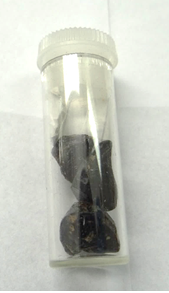
\includegraphics[width=\linewidth]{Lakshminarayanan_Figure_08}
	\caption{Roman glass fragments\\
		{\normalfont\scriptsize\copyright\ Courtesy of the UCL Institute of Archaeology Collections.
	}}
	\label{fig:Lakshminarayanan_Figure_08}
\end{figure}

A distinctive pottery named ‘Rouletted Ware’ was also found on the site (\cref{fig:Lakshminarayanan_Figure_09}). Two models were proposed by Wheeler and Begley respectively for explaining the genesis of this type. Wheeler hypothesised that better examples of this ware were imported while those made of softer fabric and Coarse material were locally-made imitations \parencite[][149]{wheeler1954}. He suggested that imitations of this technique were based on Greco-Roman techniques of chattering or rouletting. Wheeler further stated that the presence of this type of ware shows the influence of Roman trade on local production. Begley, on the other hand, noted that the ware dated prior to trade with Rome but was still influenced by Hellenistic pottery types \parencite[][427]{begley1988}.

Based on the stratigraphical analysis, the rouletted ware fragments do predate the Arrentine ware finds and is thus unlikely that it derived its inspiration from the Roman design. Instead, it is possible to suggest that the earliest production of this ware may have begun in Southern India \parencite[][54]{begley1986}.

%FIGURES 09-11: Rouletted ware
\begin{figure}[!htb]
	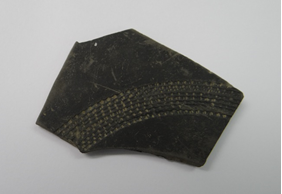
\includegraphics[width=\linewidth]{Lakshminarayanan_Figure_09}
	\caption{Fragments of Rouletted ware\\
		{\normalfont\scriptsize\copyright\ Courtesy of the UCL Institute of Archaeology Collections.
	}}
	\label{fig:Lakshminarayanan_Figure_09}
\end{figure}

The decorations and motifs inscribed on the Coarse ware were possibly a result of the strong influence of trade. The walls of the Coarse ware sherds were thicker and the fabric contains stone inclusions that are not found in Rouletted ware sherds. The Coarse ware pottery fragments show the presence of this type in tableware dishes and bowls, and large storage jars (\cref{fig:Lakshminarayanan_Figure_12} and \cref{fig:Lakshminarayanan_Figure_13}).

%FIGURE 12-13: Coarse ware
\begin{figure}[!htb]
	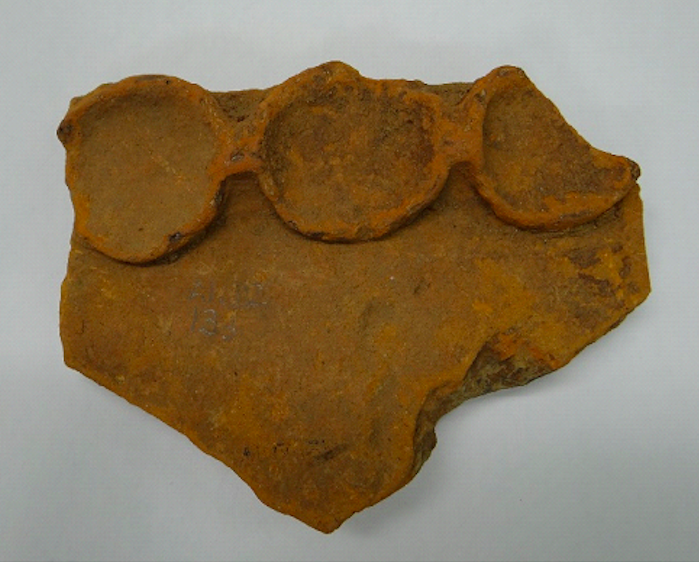
\includegraphics[width=\linewidth]{Lakshminarayanan_Figure_12}
	\caption{Coarse ware sherd\\
		{\normalfont\scriptsize\copyright\ Courtesy of the UCL Institute of Archaeology Collections.
	}}
	\label{fig:Lakshminarayanan_Figure_12}
\end{figure}

Several numismatic finds have also been identified in and around the site. Although these artefacts are not within the scope of this archaeological study, it is worth mentioning them in order to understand the significance of Roman trade in the Indian peninsula. The hoards in the peninsula are from the areas of Chennai, Hyderabad, Mysore, Cochin, Pudukkottai, and Thiruvananthapuram \parencite[][]{turner2016}. This hoard contained \emph{aurei} and \emph{denarii} from the reign of Augustus and Tiberius. During Nero’s reign in\AD 63, the Roman coin was reduced in its weight for value debasement \parencite[][68]{lannoye2015}. Significant modifications were made to the silver and gold coins during this time. The Roman currency was used as bullion, and there was no native currency that was approximated to the Roman coins. The coins were used as weight measures for gold or silver ornaments and other precious metals \parencite[][167]{wheeler1955}.

Although imported finds have been identified on site, it is hard to provide a complete picture of the significance of these imported finds because excavations were not extensively undertaken. Roman amphorae have been iden during surface surveys in sites close to Arikamedu (see \cref{fig:Lakshminarayanan_Figure_01}). Archaeological surveys in Alangankulam have identified Roman pottery and coins from the late fourth century and the fifth century\AD
\parencite{kasinathan1994}.
% \parentext{%
% 	\citeyear{kasinathan1996}}.
Similar assemblages have been identified in Coimbatore \parencite[][244]{tchernia2016}, Vasavasamudram \parencite[][133]{champakalakshmi1996}, Karaikadu \parencite[][111]{ramachandran1980} and other nearby sites. Systematic analysis of find distribution patterns could reveal more information about the quantity and the workmanship of imported objects.

\IJSRAsection{Literary and Archaeological analysis of exports}

Pliny (\emph{NH} XXXVI 20), \emph{Periplus} (\emph{PME} 49,55), and Strabo (\emph{Geo}.XV.I.67) refer to the high quality of glass manufactured in India. Pounded quartz used for glassmaking in India ensured that superior quality glass beads were produced. There was also a thriving bead-making industry identified in the archaeological record on the basis of fragments of glass and stone beads found in the industrial area of Arikamedu.

According to the \emph{Periplus}, agate and carnelian were also exported from Ratnapur, India \parencite[][127]{chandra1977}. Both worked and unworked fragments of carnelian and white agate (\cref{fig:Lakshminarayanan_Figure_14} and \cref{fig:Lakshminarayanan_Figure_15}) have been found in Arikamedu. Agate/onyx blanks of this type were likely exported to Rome to be cut into cameos \parencite[][181]{sidebotham2008}. A fragment of crystalline quartz shows that drill bits were used to partially drill a hole into the stone \parencite[][]{gwinett1988}.

%FIGURE 14: Carnelian unworked
\begin{figure}[!htb]
	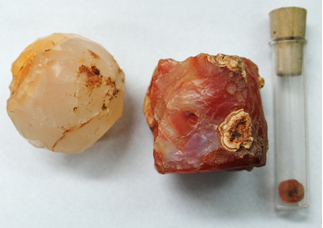
\includegraphics[width=.32\linewidth]{Lakshminarayanan_Figure_14}
	\caption{Unworked carnelian fragments and finished bead\\
		{\normalfont\scriptsize\copyright\ Courtesy of the UCL Institute of Archaeology Collections.
	}}
	\label{fig:Lakshminarayanan_Figure_14}
% \end{figure}
%
\hfill
% %FIGURE 15: Mauve glass
% \begin{figure}[!htb]
	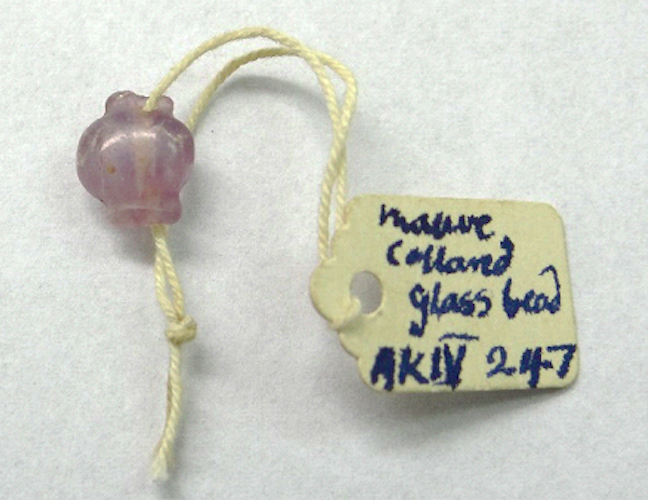
\includegraphics[width=.32\linewidth]{Lakshminarayanan_Figure_15}
	\caption{Mauve Collar glass bead\\
		{\normalfont\scriptsize\copyright\ Courtesy of the UCL Institute of Archaeology Collections.
	}}
	\label{fig:Lakshminarayanan_Figure_15}
% \end{figure}
\hfill
% %FIGURE 16: Carnelian finished
% \begin{figure}[!htb]
	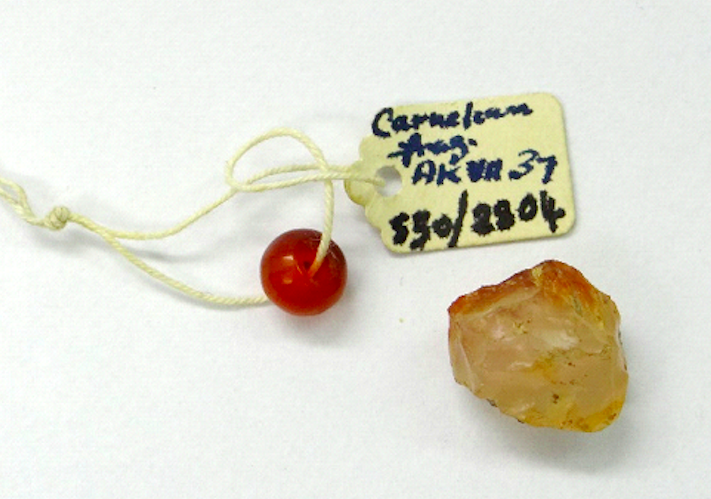
\includegraphics[width=.32\linewidth]{Lakshminarayanan_Figure_16}
	\caption{Carnelian bead finished\\
		{\normalfont\scriptsize\copyright\ Courtesy of the UCL Institute of Archaeology Collections.
	}}
	\label{fig:Lakshminarayanan_Figure_16}
\end{figure}

Collar beads were the most popular beads made in India between 400\BC and 200\AD \parencite[][117]{francis1986}. Glass tubes were used as raw stock. They were heated and then subsequently flattened to make the beads. The ends of the glass were pinched to create the shape of the bead (\cref{fig:Lakshminarayanan_Figure_16}).

According to the data available, red was the predominant colour for beads produced at the site. Carnelian was not naturally found in red colour. Chalcedony with iron content was heated to induce the red colouring in carnelian (\cref{fig:Lakshminarayanan_Figure_17}). This also suggests knowledge of production and modification techniques, as well as customisation.

%FIGURE 17: Red
\begin{figure}[!htb]
	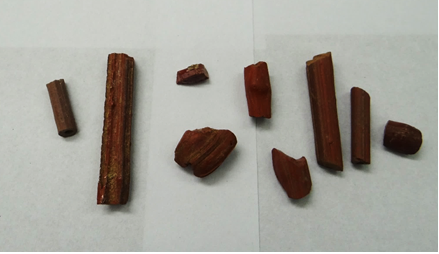
\includegraphics[width=\linewidth]{Lakshminarayanan_Figure_17}
	\caption{Red bead slag fragments\\
		{\normalfont\scriptsize\copyright\ Courtesy of the UCL Institute of Archaeology Collections.
	}}
	\label{fig:Lakshminarayanan_Figure_17}
\end{figure}

The quality of finished beads and the various techniques used to produce them suggest that workers were highly skilled. The presence of furnaces, tools, and slag at the site indicates the existence of large-scale bead production at the site. The production of beads was not only tailored to meet the demands of the Roman mercantile trade; beads were also shipped to Thailand and Sri Lanka \parencite[][4-5]{francis1990}. Similar assemblages were also found in Go Oc Eo in Vietnam in the Indo-Pacific (\cref{fig:Lakshminarayanan_Figure_18}), which might suggest that bead-making techniques from India were introduced eastwards along with the beads themselves \parencite[][17]{francis1990}.

%FIGURE 18: Map SE Asia
\begin{figure}[!htb]
	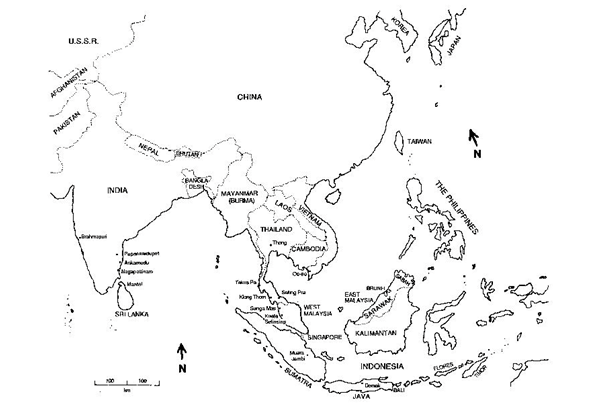
\includegraphics[width=\linewidth]{Lakshminarayanan_Figure_18}
	\caption{Map of South and East Asia. The sites shown on the map are confirmed or possible centres of Indo-Pacific bead making, in Francis (2002)\\
		{\normalfont\scriptsize\copyright\ Courtesy of Asian Perspectives
	}}
	\label{fig:Lakshminarayanan_Figure_18}
\end{figure}

Finished coloured beads of various sizes have also been found on the site (\cref{fig:Lakshminarayanan_Figure_16}). At Arikamedu, minerals such as agate, carnelian, rock crystal, amethyst, black chalcedony and garnets were used for export and local use. The stones were locally sourced from the Krishna-Godavari basin \parencite[][37]{newbold1844}, the Deccan trap, and around Hyderabad \parencite[][535]{sinkankas1996}.

If the pottery for local use found at Arikamedu was indeed an imitation of Roman types and the assemblage can be considered to reflect intensive trading activities between Arikamedu and Rome, then the economic implications of Indo-Roman trade on the imperial treasury may have been considerable. The payment for luxury goods that were imported along with any bulk goods brought to and from India appears to have cost a significant amount of money. Pliny and Tacitus both show concerns about the outflow of money into foreign countries in the context of trading (Tacitus \emph{Annales} III: 53; Pliny \emph{NH} VI: 23, \emph{NH} XII: 47). However, based on \emph{Periplus}, it can be ascertained that the trade with India was based on barter exchanges rather than extensive monetary payments. Although monetary payments were made (to some extent) in cash or bullion, the purchase of wine, \emph{garum}, and other items from the Empire by merchants in the Indian subcontinent would not have necessarily resulted in a trade deficit. At the same time, it is worth noting that the accounts made by Pliny and Tacitus were based on a moral judgement rather than government policy. These arguments were primarily directed against the vices of \emph{mollitia} and \emph{luxuria} of Roman elites, and thus they may not have been truly indicative of real economic concerns.

Trade with Arikamedu seems to have been conducted by private merchants with little to no involvement from the Roman government or from local Tamil powers. The literary and archaeological records do not show any concrete evidence of governmental influence on the trade. The archaeological record also shows that there were no restrictive product monopolies. For example, textile and gems were also purchased from Arabia as well as India. The market was able to support trade via different routes and places; thus, prices alone may not have determined the selection of the supplier, but they could have contributed to the prolonged continuity of trade.

\IJSRAsection{Internal trade}

Internal trading networks are rarely discussed in studies of Indo-Roman trade. However, due to economic demands, internal and external trading networks in the subcontinent worked simultaneously (\cref{fig:Lakshminarayanan_Figure_19}). The needs of both local and international trade led to the formation of transport networks between the source regions, industries and ports. Items that were not available in Arikamedu were likely brought in from other regions in India. At the same time, some of the items procured from Arikamedu were probably bought and sold multiple times on their way to Rome.

%FIGURE 19: Roman coins
\begin{figure}[!htb]
	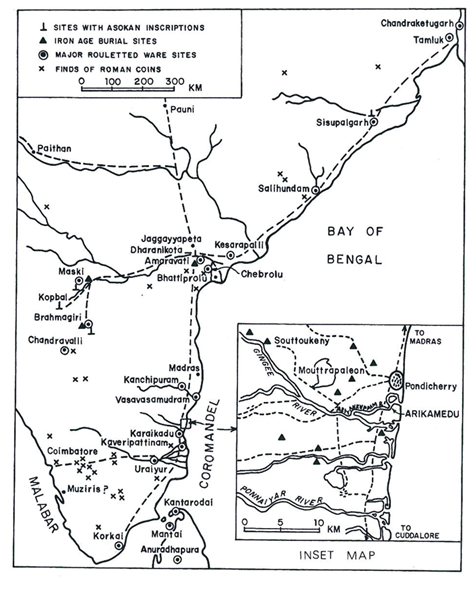
\includegraphics[width=\linewidth]{Lakshminarayanan_Figure_19}
	\caption{Distribution of Roman coins in India (Begley 1983, fig. 1)\\
		{\normalfont\scriptsize\copyright\ Courtesy American Journal of Archaeology and Archaeological Institute of America
	}}
	\label{fig:Lakshminarayanan_Figure_19}
\end{figure}

A number of goods were made from locally available materials at Arikamedu and others were made of non-local materials, such as shells from inland areas. Fragments of shell from marine life were found on site and across the hinterland. The \emph{Turbinella pyrum} was naturally distributed along the southeastern coast of India \parencites[][141]{smith2002}[][]{nagappan1974}. These typeswere used for making ornaments and bangles. The rounded portion of the shell was sawed into the shape of a bangle. These shell fragments possess a distinctive shape, thus enabling archaeologists to identify their provenance in the archaeological record. Despite the significance of the finds, the involvement of local artisans and local transportation of complete shells is yet to be assessed. Sites in the Coimbatore region and Karur show the existence of shell fragments as well as imported coinage, suggesting a strong connection with the trading network \parencite[][26]{kamalakar2000}.

Raw materials for the beads manufactured at Arikamedu were transported from other adjoining regions. Beads such as black onyx, carnelian, and banded agate were sourced from the Godavari and Krishna rivers \parencite[][115]{francis2002}. Precious and semi-precious stones such as lapis lazuli, agate, and carnelian, not available in abundance locally, were likely to have been transported from long distances and moved to the manufacturer. For example, lapis lazuli was found in abundance in Badakshan and not locally \parencite[][29]{mairs2016}.

These beads were not only traded within the Roman provinces but also along the trade route in Burma, the Isthmus of Kra, Gulf of Thailand and islands of Indonesia, together with other sites along this route \parencite[][106]{howard2012}. Collar beads were discovered in the Indonesian site of Gilimanuk \parencite[][46]{francis2002}. Rouletted ware from the site was also imported to Indonesia \parencite[][229]{ardika1991}. It can be concluded that Arikamedu played a significant role in the trade with South Asian islands; at the same time, one cannot minimise the effect of Sri Lanka and other Southern Indian trading stations on the rest of Asia \parencite[][46]{francis2002}. For example, although Arikamedu was one of the largest producers of beads, Muziris was known for exporting beads and gems. This suggests that beads were manufactured at Arikamedu and shipped to Muziris to be exported along the Roman route.

\IJSRAsection{Egyptian Network}

Egypt was a key location in the context of Indo-Roman trade. Some Roman traders operated exclusively within the Indian Ocean, following a diversity of sea routes to reach the different ports where luxury goods such as precious metal and necessity goods such as wheat and cotton were procured and traded. The journey from the ports took a stipulated travel time due to the nature of the monsoons, which was noted by \emph{Periplus}. The unique nature of the trade rendered itself to the formation of trade networks between Arabia, Africa and India. The port of Myos Homos (Egypt) was created to facilitate trade in Africa for procuring war elephants. The Ptolemaic port of Berenike was established to facilitate trade between Egypt and Aegean Islands, particularly Rhodes, in the mid third century \BC \parencite[][203]{tomber2012} The strategic location of these two ports was no doubt crucial in forming a trading network within the ports of the Indian Ocean. After the annexation of Egypt in 30 \BC, there was a large-scale increase in international trade, largely involving these ports.

A number of items found in the excavations suggest that Berenike was part of a vast network of Roman trade routes. Ostraca excavated from a rubbish dump have given two precise dates: 6 August 33 and 20 September 61. The rubbish accumulated around c. 40/5 and 70/5 based on the other ostraca finds in the area. The finds suggest that the accumulation is part of the Berenike custom station, revealing a list of traded goods, such as wine, for export and consumption \parencite[][7]{bagnall2000}. The Egyptian Dressel type 2-4 amphorae were identified along with other Mediterranean amphorae types found at Arikamedu, Pattanam, and Alangankulam located in Southern India. This network shows that trade was organised around ports, which channelled goods from producers to other agents involved in their subsequent distribution.

Quesar-al-Qadim is an important trading port in the Indo-Roman trade route, identified as Leukos Limen. Excavations conducted in Quesar Al Qadim also revealed two ostraca dating to the first century which mentions tamil names such as \emph{Kannan} and \emph{Catan}. The Berenike excavations have also revealed two ostraca written in Tamil script \parencite[][264]{whitcomb1982}.

Traded Indian beads of copper-red colour have been located in several sites along the East African coast, and can be dated to the first and second century\AD. There were several opaque red, green (\cref{fig:Lakshminarayanan_Figure_20}) and yellow beads located in Zanzibar which were typologically and chemically analysed, suggesting an Indian provenance \parencite[][33-44]{chami2001}.

%FIGURE 20: Green
\begin{figure}[!htb]
	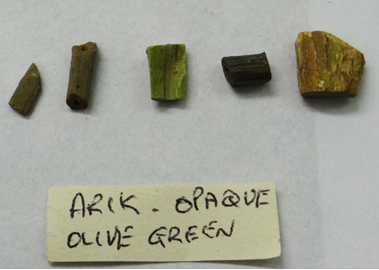
\includegraphics[width=\linewidth]{Lakshminarayanan_Figure_20}
	\caption{Opaque green bead fragments\\
		{\normalfont\scriptsize\copyright\ Courtesy of the UCL Institute of Archaeology Collections.
	}}
	\label{fig:Lakshminarayanan_Figure_20}
\end{figure}

The network of trade established by the Roman Empire not only created a market for goods in the West but also contributed to the establishment and consolidation of mercantile ports and communities along the trade route. This ensured that all types of goods were exchanged, meeting several demand requirements and creating flourishing ports for shipbuilding and maintenance. Along both sea routes mentioned in the \emph{Periplus}, intensive trade networks developed over time, due to the intertwined relationship between production areas and trading ports in the context of expanding exchange networks. Articles procured by traders at Arikamedu did not only reach the Roman world but were also sold in Egyptian and Southern Asian ports. Internal trade also expanded, partly in order to acquire raw materials and minerals for producing finished goods.

\IJSRAsection{Conclusion}

From the archaeological assemblage found at the site, it can be concluded that Arikamedu was a flourishing trading station in Southern India. The artefacts found in the different periods of occupation suggest that although trade with the Roman world was prevalent in the first century, the trading port operated for centuries, both before and after the Augustean era. The evidence in ancient literature is not extensive enough to conclusively assess the nature of this trade. Besides, Tamil literature does not particularly lend itself completely to this kind of analyses, due to issues regarding the accurate dating of the texts. It can certainly be used to confirm the prosperity of the foreign trade that is already remarked upon in Roman literature.

The prolonged foreign trade resulted in the importation of Mediterranean wares, but also subtle Roman influences in the consumption of particular products, such as wine, and other potential associated implications in terms of social norms. From a quantitative perspective, the assemblage does not necessarily reflect the entire quantity of imports. The northern sector of the site has been submerged under the river, hence the full picture of the site is currently unavailable. Influence of Roman wares on local Coarsewares can also be observed in Arikamedu. Stamped Coarse ware fragments showing influences from the Arrentine ware suggest that Mediterranean pottery types were popular in the region.

The merchants imported a number of goods from the site. Some goods were produced locally, whilst others were brought into the sites from inland areas. Beryls and gems such as amethyst were not locally found, and shells were moved from the inland regions and exported internationally. The archaeological record in India regarding perishable edible products such as spices is almost non-existent. The presence of Indo-Pacific beads found in Indonesia and South-East Asian islands suggests that Arikamedu was not only an important mercantile port for Roman trade but it was also part of broader exchange networks involving multiple Asian regions during the first century\AD.

Perhaps the most important evidence for intensive Indo-Roman trade comes from the sites of the Red-sea region. The assemblages from Quesar-al-Qaudim and Berenike reveals that Arikamedu was an active trading port, and that Tamil merchants were involved in trading with Roman Egypt. The degree of involvement of these merchants is currently unknown and all that can be said is that there are telling similarities between the assemblages from Arikamedu and the Romano-Egyptian port sites.

Indo-Roman trade remained steady and unchanged until the third century\AD. At the end of the century, trade receded, partly due to the political and financial crisis in the Roman Empire. During the next century, the trading network was re-established with a slightly different organisation than it had been in the first century onwards.

\IJSRAsection{Acknowledgements}

I am extremely grateful for the help and guidance that Dr.~Ada Nifosi provided me at every step as my supervisor. I would like to thank the University College of London’s Institute of Archaeology for allowing me to study the Arikamedu collections. I am especially thankful to Dr Rachael Sparks of the Institute for providing me with the necessary equipment and discussing the collection with me.

\IJSRAseparator

%where to put
\IJSRAsubsection{Abbreviations}
\begin{description}
\item[PME] Periplus Maris Erythraei
\item[NH] Naturalis Historia
\item[Ov. Medic] Medicamina Faciei Feminae
\item[Geo] Geography
\end{description}

\IJSRAclosing%<---- don’t change this!
